\chapter{\IfLanguageName{dutch}{Stand van zaken}{State of the art}}%
\label{ch:stand-van-zaken}

% Tip: Begin elk hoofdstuk met een paragraaf inleiding die beschrijft hoe
% dit hoofdstuk past binnen het geheel van de bachelorproef. Geef in het
% bijzonder aan wat de link is met het vorige en volgende hoofdstuk.

% Pas na deze inleidende paragraaf komt de eerste sectiehoofding.

% Dit hoofdstuk bevat je literatuurstudie. De inhoud gaat verder op de inleiding, maar zal het onderwerp van de bachelorproef *diepgaand* uitspitten. De bedoeling is dat de lezer na lezing van dit hoofdstuk helemaal op de hoogte is van de huidige stand van zaken (state-of-the-art) in het onderzoeksdomein. Iemand die niet vertrouwd is met het onderwerp, weet nu voldoende om de rest van het verhaal te kunnen volgen, zonder dat die er nog andere informatie moet over opzoeken \autocite{Pollefliet2011}.

% Je verwijst bij elke bewering die je doet, vakterm die je introduceert, enz.\ naar je bronnen. In \LaTeX{} kan dat met het commando \texttt{$\backslash${textcite\{\}}} of \texttt{$\backslash${autocite\{\}}}. Als argument van het commando geef je de ``sleutel'' van een ``record'' in een bibliografische databank in het Bib\LaTeX{}-formaat (een tekstbestand). Als je expliciet naar de auteur verwijst in de zin (narratieve referentie), gebruik je \texttt{$\backslash${}textcite\{\}}. Soms is de auteursnaam niet expliciet een onderdeel van de zin, dan gebruik je \texttt{$\backslash${}autocite\{\}} (referentie tussen haakjes). Dit gebruik je bv.~bij een citaat, of om in het bijschrift van een overgenomen afbeelding, broncode, tabel, enz. te verwijzen naar de bron. In de volgende paragraaf een voorbeeld van elk.

% \textcite{Knuth1998} schreef een van de standaardwerken over sorteer- en zoekalgoritmen. Experten zijn het erover eens dat cloud computing een interessante opportuniteit vormen, zowel voor gebruikers als voor dienstverleners op vlak van informatietechnologie~\autocite{Creeger2009}.

% Let er ook op: het \texttt{cite}-commando voor de punt, dus binnen de zin. Je verwijst meteen naar een bron in de eerste zin die erop gebaseerd is, dus niet pas op het einde van een paragraaf.

\label{sec:grafiekmodellering}
\section{Grafiekmodellering}
Grafiekmodellering is een techniek die gebruikt wordt om de data te visualiseren en te analyseren. In deze bachelorproef wordt dit gebruikt om de verbanden te leggen tussen de verschillende processen binnen ArcelorMittal Gent.
Dit gebeurt door middel van knopen die verbonden zijn met andere knopen met een relatie. \autocite{neo4j20252}.
Een knoop stelt een entiteit voor, zoals een persoon, een product of een proces. Een verbinding stelt de relatie tussen de verschillende knopen voor zoals een associatie, transformatie of transactie van een product.
Dit kan in ons geval een staalplaat zijn die door een kraan verplaatst wordt. Hierbij zijn de kraan en staalplaat de knopen en is de verplaatsing een transactie-relatie tussen deze knopen.
Elke knoop bevat ook properties die de knoop beschrijven. Dit kan bijvoorbeeld het bouwjaar van een machine zijn of de temperatuur van een product, deze worden opgeslagen als sleutel-waarde paar om later efficiënt te kunnen ophalen.

\subsection{Cosmos DB}%
Cosmos DB is een NoSQL\-database van Microsoft. Het biedt een lage latentie, multi\-query\-API die eenvoudig grote hoeveelheden data kan verwerken en heeft een grote beschikbaarheid, zegt~\textcite{Put2020}, wat zeer belangrijk is in ons project.
Daarnaast is CosmosDB horizontaal schaalbaar, wat betekent dat we op hoogtepunten tot een miljoen lees- en schrijfaanvragen kunnen verwerken door het benodigde aantal servers toe te voegen.
De hoge beschikbaarheid wordt gegarandeerd door replicatie, waardoor we snel kunnen overschakelen als er een probleem is in onze database.
Binnen ArcelorMittal wordt gebruik gemaakt van de azure omgeving van Microsoft, waardoor CosmosDB een logische keuze is voor ons project.
CosmosDB ondersteunt verschillende API's zoals SQL, MongoDB, Cassandra, Gremlin en Table API, waardoor we flexibel kunnen werken met verschillende soorten data.
De connectie met CosmosDB gebeurt via een private endpoint, waardoor we de data veilig kunnen opslaan en allen kunnen raadplegen via het domein van op ArcelorMittal Gent.
\subsection{Gremlin API}
Gremlin is een database query taal die gebruikt wordt om te communiceren met grafiek databases zoals CosmosDB \autocite{Tinkerpop2023}.\@
De taal bevat verschillende varianten zoals Gremlin\-Java, Gremlin\-Python en Gremlin\-Groovy,\dots
In ons geval zullen we Gremlin\-Javascript gebruiken om de data van ArcelorMittal Gent in CosmosDB te bevragen. De bevraging is gebasseerd op een RestAPI die de data ophaalt en teruggeeft in JSON formaat.
Javascript is hiervoor geschikt omdat Javascript en JSON een goede combinatie zijn om data te verwerken, daarnaast maken we ook gebruik van NodeJS wat met JavaScript werkt. 
Als extra kan je met JavaScript eenvoudig front end en back end combineren, wat mogelijk is voor verdere uitbereiding van deze thesis.
Hiernaast hebben we ook Neo4J overwogen met cypher als query taal, maar deze heeft zijn eigen ecosysteem en is niet even flexibel en schaalbaar als Gremlin API.\@
Gremlin daarentegen voorziet dat alle databases die TinkerPop\-enabled zijn, kunnen worden gebruikt. Hieronder vallen onder andere Amazon Neptune, CosmosDB, JanusGraph en nog vele andere.\autocite{Tinkerpop2023a}

\subsection{NodeJS}
NodeJS is een open\-source JavaScript runtime\-omgeving die de mogelijkheid biedt om JavaScript\-code uit te voeren op de server ~\autocite{NodeJS2022}.
Dit gebeurt via een Single\-Threaded, Non\-Blocking I/O model wat betekent dat er geen nieuwe threads worden aangemaakt voor elke request.
Door middel van Callbacks en Promises werkt NodeJS asynchroon, wat betekent dat de code niet wacht op een antwoord van een request maar ondertussen andere requests kan verwerken.
Met event loops worden de requests in een wachtrij geplaatst en worden ze verwerkt wanneer de server klaar is met een andere operatie.
Daardoor is NodeJS zeer performant en schaalbaar voor het verwerken van grote hoeveelheden data.

De technologie is in 2009 ontwikkeld en geïntroceerd door Ryan Dahl en is sindsdien zeer populair geworden in de webontwikkeling. 
NodeJS werd later door grote bedrijven zoals Netflix, eBay \& Uber gebruikt voor hun back-end systemen.
Zoals eerder vermeld is het geen framework maar een runtime\-omgeving, dit betekent dat het geen standaardbibliotheken heeft die hergebruikt kunnen worden door developers.
Dit biedt volledig vrijheid in hoe de architectuur van de applicatie wordt opbouwt.

Een van de nadelen van NodeJS is dat het single\-threaded is, wat betekent dat het niet geschikt is voor CPU\-intensieve taken.
Dit komt omdat NodeJS gebruik maakt van een event loop die de requests in een wachtrij plaatst en ze verwerkt wanneer de server klaar is met een andere operatie.
Hierdoor kan het zijn dat een request die veel tijd nodig heeft om te verwerken de andere requests blokkeert.
Sinds 2018 is er een nieuwe feature geïntroduceerd in NodeJS genaamd Worker Threads, dit maakt het mogelijk om multi\-threaded te werken.
Daardoor kunnen we de CPU\-intensieve taken in een aparte thread verwerken en de main thread vrij houden voor andere requests.

\subsection{EPCIS-events}
Voor dit onderzoek maken we gebruik van EPCIS (Electronic Product Code Information Services), dit is een GS1\-standaard die bedrijven in staat stelt om gebeurtenissen in de toeleveringsketen vast te leggen en te delen. 
Het biedt een gemeenschappelijk kader voor het vastleggen van de wat, wanneer, waar en waarom van gebeurtenissen die betrekking hebben op fysieke of digitale objecten. 
Deze waarden zijn ontwikkeld door GS1 om gegevens over beweging, status en verandering van een item in de toeleveringsketen (supply chain) vast te leggen en te delen binnen en buiten het bedrijf \autocite{Devins}.
``Met behulp van deze waarden kunnen we real\-life objecten omzetten in elektronisch opgeslagen informatie, waarna we dit kunnen communiceren met eindgebruikers.`` zegt \textcite{Devins}.
Door deze normen toe te passen kunnen we de traceerbaarheid van het product per proces garanderen inclusief de gewenste parameters die opgeslagen worden in ons grafiekmodel zoals tijd (wanneer) en temperatuur (hoe), waar nodig.
Voor deze relaties goed en volgens de normen op te stellen, maken we gebruik van de EPCIS\-events. Dit is een referentielijst waarin verschillende acties vooraf zijn bepaald.
Hier hebben we bijvoorbeeld acties zoals ``add'', ``delete'' en ``update'' die we gebruiken om de data te structureren.
De add\-actie wordt gebruikt om een nieuwe knoop toe te voegen aan het grafiekmodel, de delete\-actie om een knoop te verwijderen en de update\-actie om een knoop bij te werken.
Bij deze actie voegen we ook properties toe in een event\-lijst, daar bepalen we welk soort event we gebruiken en voegen we eventueel extra parameters toe voor op de relatie, zoals tijd.


De belangrijkste voordelen volgens \textcite{GS12025} staan opgelijst in tabel~\ref{tab:epcis-voordelen}.
\begin{table}[H]
    \centering
     \begin{tabular}{lp{0.6\textwidth}}
          \toprule
          \textbf{Voordeel} & \textbf{Beschrijving} \\
          \toprule
          Verbeterde zichtbaarheid & Door het vastleggen en delen van gedetailleerde gebeurtenisgegevens kunnen bedrijven beter inzicht krijgen in de bewegingen en status van producten in de toeleveringsketen. \\
          \midrule
          Efficiëntieverbeteringen & Door het automatiseren van gegevensverzameling en \-uitwisseling kunnen bedrijven operationele efficiëntie verbeteren en fouten verminderen. \\
          \midrule
          Naleving van regelgeving & EPCIS helpt bedrijven te voldoen aan wettelijke vereisten voor traceerbaarheid en rapportage. \\
          \midrule
          Betere samenwerking & Door het delen van gebeurtenisgegevens met partners kunnen bedrijven beter samenwerken en de toeleveringsketen optimaliseren. \\
          \bottomrule
     \end{tabular}
     \caption[Belangrijkste voordelen van EPCIS volgens GS1]{\label{tab:epcis-voordelen}}
\end{table}

\subsection{GS1}
GS1 is een wereldwijde organisatie die standaarden ontwikkelt voor identificatie, codering \& uitwisseling~\autocite{GS1standards}.
Dit zijn standaarden die bedrijven helpen om hun producten en diensten te identificeren, traceren en uit te wisselen.
Elk product heeft een unieke identificatiecode die het mogelijk maakt om het product te traceren doorheen de toeleveringsketen.
GS1 heeft verschillende standaarden ontwikkeld zoals de GTIN\-code (Global Trade Item Number), GLN\-code (Global Location Number) en SSCC\-code (Serial Shipping Container Code).
De GTIN\-code is een code voor producten, elk product dat traceerbaar wil zijn moet een GTIN\-code hebben. 
Indien de GTIN niet aanwezig is kunnen er verschillende stappen ondernomen worden, in figuur~\ref{fig:gtin} is een overzicht te zien van de verschillende stappen die ondernomen kunnen worden.
Ook locaties kunnen een unieke code krijgen, dit is dan de GLN\-code. In volgende secties gaan we dieper in op de ontwikkeling van de GTIN\-code en de GLN\-code.

\subsubsection{GTIN}
De GTIN\-code ofwel het Global Trade Item Number is een unieke identificatiecode die wordt gebruikt om producten te identificeren in de toeleveringsketen \autocite{GTIN2025}.
Deze bestaat uit 7 tot 11 cijfers benoemd met GTIN\-8, GTIN\-13 en GTIN\-14, de groote van de code hangt af van de toepassing en het type product.
Producten die klein zijn en weinig informatie bevatten kunnen een GTIN\-8 hebben, terwijl grotere producten zoals dozen of pallets een GTIN\-14 kunnen hebben.
In de gezondheidszorg wordt vaak een GTIN\-14 ook toegelaten aangezien er ook veel informatie nodig kan zijn voor bijvoorbeeld medicatie.
De opbouw van de code is vrij simpel: de eerste 7 tot 11 cijfers identificeren jouw bedrijf, hoe korter deze prefix is, hoe meer producten je kan identificeren.
Na deze code volgt de productcode, dit is ook een reeks unieke cijfers voor identificatie van het product.
Als laatste volgt het controlecijfer, dit is een cijfer dat wordt berekend op basis van de andere cijfers in de code.
Dit cijfer wordt gebruikt om te controleren of de code correct is ingevoerd en of er geen fouten zijn gemaakt bij het scannen van de code.

\begin{figure}[h]
     \centering
     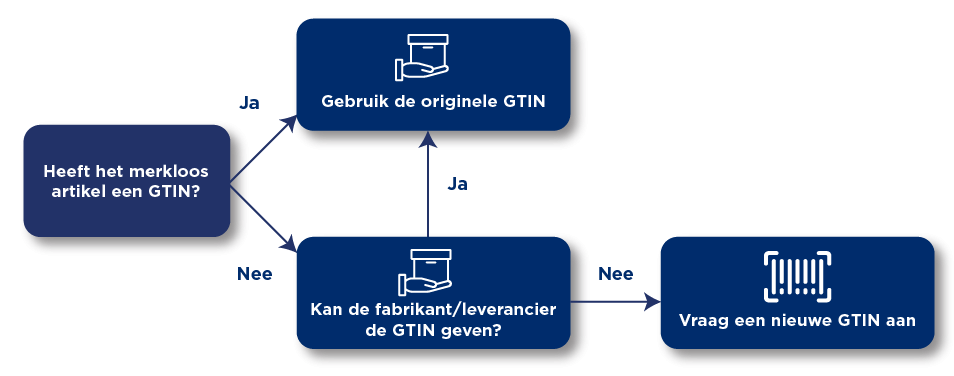
\includegraphics[width=0.8\textwidth]{./img/GTIN.png}
     \caption[GTIN stappenplan]{\label{fig:gtin} GTIN stappenplan. Geraadpleegd op~\cite{GTIN2025} }
\end{figure}

\subsubsection{GLN}
De GLN\-code ofwel het Global Location Number is een unieke identificatiecode die wordt gebruikt om locaties te identificeren in de toeleveringsketen \autocite{GLN}.
Deze code is vergelijkbaar met de GTIN\-code maar wordt gebruikt voor locaties, de opbouw daarentegen is gelijkaardig.
De GLN code moet sinds 1 juli 2022 een uniek cijfer zijn en mag niet hergebruikt worden voor andere locaties.
De opbouw is zoals eerder vermeld gelijkaardig, eerst hebben we de bedrijfsprefix, daarna volgt het adresnummer en als laatste een controlecijfer.
De bedrijfsprefix is een unieke code die wordt toegekend aan jouw bedrijf, deze code kan je aanvragen bij GS1. Het adresnummer is een unieke code die wordt toegekend aan jouw locatie, dit kan bijvoorbeeld een gebouw of een afdeling zijn.


\subsection{Schema.org}
Schema.org is een grote verzameling van gestructureerde data die entiteiten (knopen) en relaties kan weergeven ~\autocite{Douglas2023}.
Je kan schema.org vergelijken met GS1 maar dan meer generiek. In ons project zullen we de combinatie van schema.org objecten en GS1 objecten gebruiken om de data te structureren.
Om een voorbeeld te geven hebben we in de data gebruik gemaakt van een splitsing tussen locaties en assets.
Elke locatie krijgt een type, een label en extra properties zoals een adres of een geografische locatie.
Dit type of ID kan bijvoorbeeld ``Place'' zijn voor een locatie of ``Product'' voor een asset. 
Op de website van schema.org zijn alle mogelijkheden beschikbaar om de data te structureren en te annoteren.
Daardoor houden we een duidelijk onderscheid tussen de soorten afdelingen en machines binnen de afdeling.
In codefragment~\ref{fig:jsonld} is een voorbeeld te zien van een JSON\-LD bestand met gegevens volgens Schema.org.
Voor de locatie van Gent hebben we ID 123, is het type een plaats en kunnen we de vorige knoop teruggeven met containedInPlace.
Verder kunnen properties toegevoegd worden zoals eronder aangegeven met een key-value paar.
% In het codeblok \ref{lst:jsonld} is een voorbeeld te zien van een JSON\-LD bestand met gegevens.
\begin{listing}
     \begin{minted}{jsonld}
          {
          "@context": "https://schema.org",
               "@graph": [
                    {
                         "@id": "123",
                         "@type": "Place",
                         "name": "Gent",
                         "label": "Gent",
                         "containedInPlace": 321,
                         "KEY": "VALUE"
                         
                    },
               ]
          }
     \end{minted}
     \caption[Voorbeeld JSON\-LD bestand]{\label{fig:jsonld}Voorbeeld van een JSON\-LD bestand met locatiegegevens.}
\end{listing}

\section{Data preprocessing}
De data die we gebruiken komt uit een SAP systeem. Deze data bevat een functionele boom structuur van de verschillende levels binnen ArcelorMittal Gent.
Dit houdt in dat de data in een hiërarchische structuur is opgebouwd, waarbij de verschillende processen met elkaar verbonden zijn.
Voor het ontcijferen van deze data hebben we verschillende specialisten binnen ArcelorMittal gecontacteerd die ons hebben geholpen met het vertalen van de datacodes.
Alleen voor deze opsplitsing tussen locatie en machine is er een grote moeilijkheid. Normalieter zou deze SAP data opgeplitst zijn zodat level 1 en level 2 de afdelingen zijn en vanaf level 3 machines. 
Helaas is in dit onderzoek geen garantie dat dit klopt, na controle lijkt dit voor 80\% van de data te kloppen, maar als een afdeling uitgebreider is kan dit verschillen.
Doordat de data enorm groot is waardoor handmatig opsplitsen eindeloos werk is en er geen garantie is op deze splitsing gaan we er vanuit dat het wel klopt dat level 2 de splitsing is. 
Dit betekent dat er voor verdere integratie een structurele aanpassing moet gebeuren aan de dataset.
Zo gaan we er van uit dat level 1 in de boom de site zelf is en dat level 2 de verschillende afdelingen zijn binnen de site. Zo gaat het telkens dieper tot level 12 waar de verschillende onderdelen van de machines zich bevinden.
Elke machine heeft een unieke code die we uit een dictionairy kunnen halen die we hebben ontvangen van ArcelorMittal.
Deze ontcijferingen zijn nodig in een later proces om onze chatbot een correct antwoord te laten geven op de vragen van de gebruiker.

\subsection{JSON tot Graph}
De data die we ontvangen van ArcelorMittal uit SAP is in JSON formaat. Deze data stelt ons in staat om door de beschrijving van de keywords de data te ontcijferen en te verwerken in ons grafiekmodel.
Omdat wij voor Gremlin en EPCIS werken met schema.org hebben wij een JSON\-LD formaat nodig. Dit is een uitbreiding van JSON die het mogelijk maakt om data te structureren en te annoteren.
Daarna kunnen we deze JSON\-LD in een folder plaatsen en wordt deze automatisch ingelezen met een NodeJS script.
Deze gaat voor alle types een knoop aanmaken en de bestaande properties toevoegen aan de JSON\-LD.\@ Hierbij kunnen we nog bepalen welke properties we gebruiken en zelf de key van de properties bepalen.
Daarna kunnen we ook de relaties aanmaken volgens de schema.org structuur, dit gebeurt door de huidige knoop ID te verbinden met het ID van de parent, deze zitten ook in de SAP data verworven en kunnen dus makkelijk eruit gehaald worden.
Om de relaties te bepalen maken we gebruik van het hierarchisch level. Deze property bepaald of het een locatie is, een machine of onderdelen van de machine, in onze terminologie noemen we dit ook wel de assets.
Door de combinatie van het level en de parent kunnen we zelf bepalen in de vertaling van JSON naar JSON\-LD welke relatie op welk level gebruikt kan worden.

\begin{figure}[h]
     \centering
     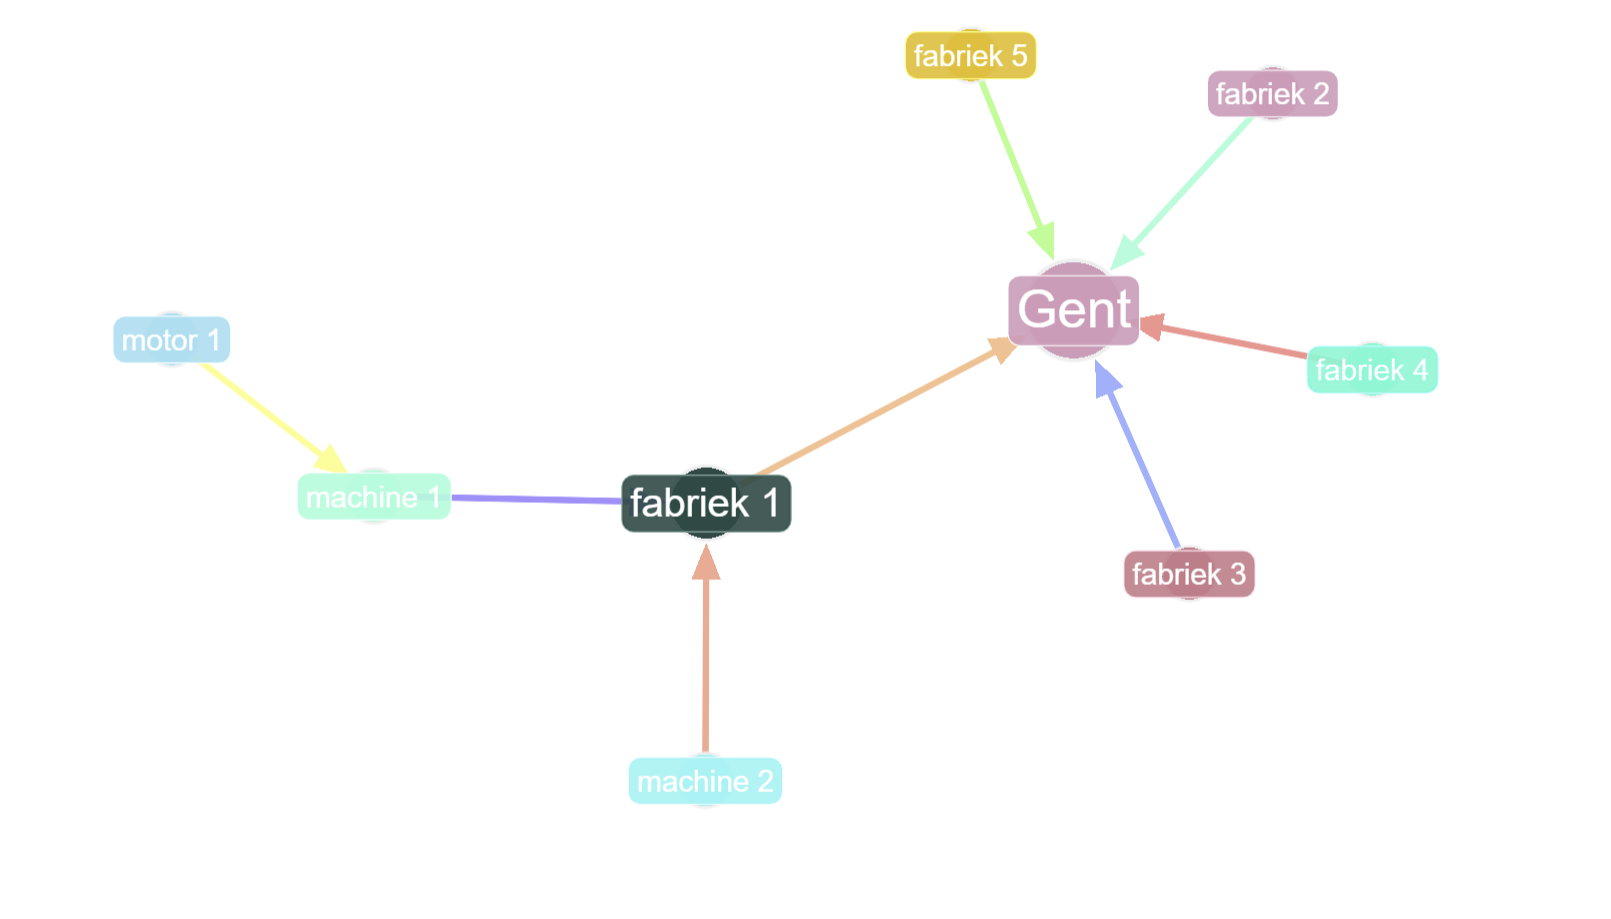
\includegraphics[width=0.8\textwidth]{./img/grapmodel_example.png}
     \caption[Voorbeeld Grafiekmodel.]{\label{fig:graphmodel}Voorbeeld van kleinschalig grafiekmodel, gemaakt met mock data.}
\end{figure}


\section{Chatbot}
Een chatbot is in ons geval een API die geintegreerd kan worden in onder andere Teams. Deze chatbot kan vragen beantwoorden over de data die in het grafiekmodel zit.
Door het versturen van een Post request naar de chatbot API begint het achterliggende werk waar we hieronder dieper op in gaan. 

\subsection{Ollama}
Voor ons lokaal model maken we gebruik van Ollama. Dit is een open-source bibliotheek die verschillende vooraf getrainde modellen bevat. 
Dat is een groot voordeel omdat we in deze thesis de scope niet leggen op het maken van een large language model die natuurlijke taal kan verwerken.
Wel zijn we op zoek moeten gaan naar het beste model voor het maken van Gremlin queries. Dit is geen eenvoudige klus, dit omdat er verschillende Gremlin versies bestaan die een andere query syntax hebben.
Dit kan dus resulteren in queries die niet uitvoerbaar zijn in onze CosmosDB.\@
Tijdens de testfase zijn er verschillende modellen getest geweest, zoals llama2, llama3, gemma \& Phi4.
De llama modellen waren heel goed in het omzetten van de uitvoer naar natuurlijke taal, maar hadden veel moeite met het omzetten van de input naar een Gremlin query.

% Een voorbeeld van een JSON-LD bestand is te zien in listing \ref{lst:jsonld}.
% Hierin zien we dat er een type is van ``Place'' en dat er een naam is van ``ArcelorMittal Gent''.
% \begin{figure}
%   \centering
%   
\includegraphics[width=0.8\textwidth]{grail.jpg}
%   \caption[Voorbeeld figuur.]{\label{fig:grail}Voorbeeld van invoegen van een figuur. Zorg altijd voor een uitgebreid bijschrift dat de figuur volledig beschrijft zonder in de tekst te moeten gaan zoeken. Vergeet ook je bronvermelding niet!}
% \end{figure}

% \begin{listing}
%   \begin{minted}{python}
%     import pandas as pd
%     import seaborn as sns

%     penguins = sns.load_dataset('penguins')
%     sns.relplot(data=penguins, x="flipper_length_mm", y="bill_length_mm", hue="species")
%   \end{minted}
%   \caption[Voorbeeld codefragment]{Voorbeeld van het invoegen van een codefragment.}
% \end{listing}


% \begin{table}
%   \centering
%   \begin{tabular}{lcr}
%     \toprule
%     \textbf{Kolom 1} & \textbf{Kolom 2} & \textbf{Kolom 3} \\
%     $\alpha$         & $\beta$          & $\gamma$         \\
%     \midrule
%     A                & 10.230           & a                \\
%     B                & 45.678           & b                \\
%     C                & 99.987           & c                \\
%     \bottomrule
%   \end{tabular}
%   \caption[Voorbeeld tabel]{\label{tab:example}Voorbeeld van een tabel.}
% \end{table}

